\documentclass[10pt, conference, compsocconf]{IEEEtran}

% packages
\usepackage{algorithm}
\usepackage{algorithmic}
\usepackage{amsfonts} % for R symbol (the set of real numbers)
\usepackage{color}
\usepackage[pdftex]{graphicx}
\usepackage{hyperref}
\usepackage{mathtools}
\DeclarePairedDelimiter{\ceil}{\lceil}{\rceil}
\DeclarePairedDelimiter{\floor}{\lfloor}{\rfloor}

% new commands
\newcommand{\todo}[1]{
  \color{red}\emph{[#1]}
  \color{black}
}

\newcommand{\note}[1]{
  \color{blue}\emph{[Note: #1]}
  \color{black}
}


\begin{document}

\title{Sequential algorithms to split and merge terabyte-scale 3D images}

\maketitle

\begin{abstract}
  \todo{The abstract goes here. DO NOT USE SPECIAL CHARACTERS,
    SYMBOLS, OR MATH IN YOUR TITLE OR ABSTRACT.}  Authors (final order
  to be discussed when the paper shapes up): Yongping/Val\'erie,
  Yuhong Yan, Tristan. Perhaps Pierre Bellec. \note{This is a note.}
\end{abstract}


\section{Introduction}

Three-dimensional images that exceed typical memory size are
increasingly found in a variety of disciplines. BigBrain, for
instance, is a 3D histological image of the human brain that
represents 1~TB of data organized in 3600 planes at full resolution
(1$\mu$m in-plane), and 76~GB at a 40$\mu$m isotropic resolution
commonly used in neurosciences~\cite{amunts2013bigbrain}. Other
examples found in medical imaging, our primary domain of interest,
include \todo{electromicroscopy,spectroscopy-francoise-peyrin}. As
such images would typically be processed on a computing cluster,
possibly using locality-aware file systems such as HDFS, software
libraries are needed to split and merged such images efficiently. We
introduce and compare a family of algorithms to address this problem
in a sequential environment made of a single storage disk. We are
aware of the need for parallel algorithms that would split and merge
images to and from an array of disks but we plan to describe such
algorithms in a subsequent paper based on the results of the present
one.


%also in
%MB/s).

Images are split into chunks representing 3D blocks or 2D slices. We
assume that a block or slice fits in memory. The BigBrain would
perhaps be split into 125 chunks of 600~MB. The decision to split an
image into slices or blocks, and the size of the resulting chunks, may
be constrained by the application. Some applications, for instance
spatial filtering, would commonly require blocks while other ones such
as acquisition artifact removal would rather work on
slices. Flexibility is thus required in the splitting
scheme. Applications processing voxels individually, for instance
histogram computation or k-means clustering, could work on either
slices or blocks.

The main problem encountered in the context of this paper is the fact
that, if not ordered properly, data reads and writes might result in
extensive seek times that, as we illustrate below, drastically limit
the I/O performance. This problem is obviously related to the ordering
of data bytes in image files, which we assume is arbitrary but known
to the algorithm. The problem is also related to the geometry of the
chunks to extract or merge, which we again assume arbitrary but known
to the algorithm. In a nutshell, we are looking for algorithms to
reduce seek times while allowing for arbitrary chunk geometries and
arbitrary byte orders in data files. The main idea of the variations
presented in the remainder of the paper is to convert data orderings
in memory before writing them on disk. 

The literature looks remarkably scarce on the problem described
above. Parallel processing of 3D images has obviously been extensively
studied, but methods have focused more on geometrical approaches to
partition images and on load-balancing and task scheduling techniques
while we aim at algorithms to efficiently split or merge images
regardless of the geometry of the chunks \todo{do a serious literature
review on this topic}. Perhaps this lack of related works could be
attributed to the fact that disk I/O weren't a bottleneck until image
resolution reached a certain threshold. A relevant reference is the
description of the Open Connectome Data Cluster~\cite{burns2013open},
a data warehouse system that allows users to retrieve specific chunks
of large datasets. In this work, the problem of long seek times is
addressed by designing a specific file format based on space-filling
curves, that elegantly preserves spatial proximity on disk. However,
addressing the problem using a specific data organization optimizes
the system for specific chunk geometries, volumetric in this case,
while we aim at algorithms that support multiple types of geometries.

This paper makes the following contributions:
\begin{itemize}
  \item We propose a set of algorithms to split and merge 3D images
    that do not fit in memory.
  \item We model the performance (execution time) of these algorithms,
    based on a simple but realistic disk I/O model.
  \item We evaluate our model and algorithms on a representative
    use-case involving a 1~TB image a hard drive and a solid-state
    drive.
  \item We compare the algorithms in a variety of conditions based on the validated model.
\end{itemize}
Section~\ref{sec:algos} presents our algorithms and models,
Section~\ref{sec:results} details the results and
Sections~\ref{sec:discussion} discusses them.

\section{Algorithms and Models}
\label{sec:algos}

In our context, split and merge relate to the same dual
problem \todo{not so sure about this actually}. Without loss of
generality, we focus here on merging for the sake of concision. Our
goal then is to merge a set of $n$ chunks into a single reconstructed
3D image with $R$ voxels of size $b$. We assume that all chunks are of
identical size and that slices are squares and blocks are cubes.

Without loss of generality, we consider a file format where voxels are
written after alphanumerical sorting of their (x,y,z)
representation. That is, x slices are written one after the other, and
in every x slice, y rows are written one after the other. NifTI, the
file format defined by the Neuroimaging Informatics Technology
Initiative Nifti\footnote{\url{https://nifti.nimh.nih.gov}} is such a
format, used by the vast majority of the neuroimaging community. In
the remainder, we use the term ``slice" for ``x slice".

\subsection{Notations}

We adopt the following notations:
\begin{itemize}
\item $R=D^3$: number of voxels in the reconstructed image.
\item $b$: number of bytes per voxel in the reconstructed image and chunks (in B).
\item $n$: number of chunks (blocks or slices).
\item $\alpha_r$: data read rate from disk (in B/s).
\item $\alpha_w$: data write rate to disk (in B/s).
\item $\beta$: disk access time (in s).
\item $\sigma: \mathbb{R}^{+} \rightarrow \mathbb{R}^{+}$: seek time (in s), function of the seek
  distance (in B).
\item $m$: amount of available RAM (in B).
\end{itemize}

The following properties are straightforward applications of these
definitions:
\begin{itemize}
\item number of bytes per chunk: $\frac{Rb}{n}$
\item number of chunks that can fit in memory: $\frac{m.n}{Rb}$
\end{itemize}
For the sake of mathematical simplicity, the models below assume that
the reconstructed image and blocks are cubic. Under this assumption,
we have the following definitions and properties:
\begin{itemize}
\item Number of slices in a block: $\sqrt[3]{\frac{R}{n}}=d$. This is
  also the number of rows and columns in a slice and the number of
  voxel in a row or column.
\item Number of blocks required to fully cover a slice in the
  reconstructed image: $\sqrt[3]{n}^2=n^{\frac{2}{3}}$
  \item Number of full slices that can be reconstructed from $k$
    blocks: $\floor*{\frac{k}{n^{\frac{2}{3}}}}\sqrt[3]{\frac{R}{n}}$
\end{itemize}
\todo{Make a figure to illustrate the notations.}

\subsection{Disk model}

We use a simplistic disk model where a disk is characterized by its
read and write rates ($\alpha_r$ and $\alpha_w$, in B/s) and its
access time $\beta$ (in s). In particular, we assume that seeks
require a constant amount of time, regardless of the position seeked
to. In practice, large variations would be expected, but modeling such
variations would inevitably lead to models specific to the hardware,
file system or operating system, which we intentionally avoid
here. Thus, our goal is to find algorithms that minimize the
\emph{number} of seek operations. Likewise, in modern systems, read
and write times are greatly impacted by caching occurring at several
levels, which we do not model here.

%% and its seek time,
%% a function $\sigma$ of the seek distance (in B). More precisely,
%% $\sigma$ would typically be in the order of $\beta$ when an opened
%% file is seeked to a random position, but it would be much smaller when
%% a file is seeked to a nearby position.
%% The disk model encompasses file systems, kernel modules and disk
%% controllers required to access the disk from a program run in user
%% space. In modern systems, this often includes caching at various
%% levels \todo{\cite{x}}, which we will model by zeroing $\alpha_r$ or
%% $\alpha_w$ values depending on the application.

\subsection{Slices vs blocks}

Algorithms~\ref{algo:naive-slices} and~\ref{algo:naive-blocks} are the
naive merging methods for slices and blocks.
\begin{algorithm}[h]
\caption{Naive merging from slices.}
\label{algo:naive-slices} 
\begin{algorithmic}
  \FOR{each slice}
    \STATE read slice
    \STATE write slice in reconstructed image
  \ENDFOR      
\end{algorithmic}
\end{algorithm}

\begin{algorithm}[h]
\caption{Naive merging from blocks.}
\label{algo:naive-blocks}
\begin{algorithmic}
  \FOR{each block}
    \STATE read block
    \STATE write block in reconstructed image
  \ENDFOR 
\end{algorithmic}
\end{algorithm}

Algorithms~\ref{algo:naive-slices} and~\ref{algo:naive-blocks}
actually have very different performance even though blocks and slices
have identical sizes. Since slices are stored contiguously in the
reconstructed image, the number of seeks in
Algorithm~\ref{algo:naive-slices} is only $2n$:
\begin{equation}
  N_\mathrm{slices} = 2n 
\end{equation}
However,
Algorithm~\ref{algo:naive-blocks} has to do extra seeks for each row
in each slice of each block. That is, the total number of seeks
performed by Algorithm~\ref{algo:naive-blocks} is:
\begin{equation}
N_\mathrm{blocks} = 2n+nd^2 = n\left(1+\sqrt[3]{\frac{R}{n}}^2\right)
\end{equation}
In
practice, this difference could lead to a tremendous slowdown as we will show
later.

%%  For slices, the total merge time is modeled as follows:
%% \begin{equation}
%% T_\mathrm{slices} = \frac{bR}{\alpha_r}+\frac{bR}{\alpha_w}+2\beta n
%% \end{equation}
%% and for blocks:
%% \begin{equation}
%%   \begin{multlined}
%%     T_\mathrm{blocks} = \frac{bR}{\alpha_r}+\frac{bR}{\alpha_w}+ 2\beta n + \\
%%     n\left({\sigma(bR/2)} + d(d-1)\sigma\left((D-d)b\right)+d\sigma\left((D^2-d^2)b\right) \right)
%%     \end{multlined}
%% \end{equation}

\subsection{Sorted blocks}

Sorting blocks alphanumerically by (x,y,z) as shown on Algorithm 2
reduces the seek time between blocks. 

\begin{algorithm}[h]
  \caption{Merging from sorted blocks.}
  \label{algo:sorted-blocks}
  \begin{algorithmic}
    \STATE list = sort blocks according to (x,y,z)
    \FOR{each block in list}
      \STATE read block
      \STATE write block in reconstructed image
    \ENDFOR
  \end{algorithmic}
  \end{algorithm}

\todo{Not sure what we are measuring here. The number of seeks will be identical. The difference in seek time is supposed to be very minimal.}

\subsection{Buffered slices}

The algorithms presented up to now are in fact particular cases of
memory buffering where the amount of available memory equals the
maximum size of a chunk. 

\begin{algorithm}[h]
  \caption{Buffered merging from slices}
  \label{algo:buffered-slices}
  \begin{algorithmic}
    \STATE list = sort slices by increasing x values
    \STATE initialize buffer
    \STATE index = 0
    \WHILE{index\textless n}
      \WHILE{sizeof(buffer)\textless m}
        \STATE slice = list[index]
        \STATE read slice and append it to buffer
        \STATE index += 1
       \ENDWHILE
       \STATE write buffer in reconstructed image
       \STATE clear buffer
    \ENDWHILE
  \end{algorithmic}
\end{algorithm}

\begin{equation}
N_\mathrm{buff\_slices} =  n + \ceil*{\frac{bR}{m}}
\end{equation}


\subsection{Buffered blocks: Cluster reads}


As detailed in Algorithm~\ref{algo:cluster-reads}, cluster reads load
multiple blocks in memory, concatenate them in a buffer and write the
buffer sequentially in the reconstructed image. The buffer is a slightly complex
data structure, for instance an associative array or a Python
dictionary, capable of storing multiple disjoint sequences of
contiguous bytes without having to allocate memory for the bytes
between such sequences. Implementation details about the buffer are
given later in the document.

\begin{figure}
\centering
\def\svgwidth{0.3\columnwidth}
\input{figures/no-seek.pdf_tex}
\def\svgwidth{0.3\columnwidth}
\input{figures/d-seeks.pdf_tex}
\def\svgwidth{0.3\columnwidth}
\input{figures/d2-seeks.pdf_tex}
\caption{Left: complete slices and rows are reconstructed in memory:
  no seeking is required. Center: complete rows but incomplete slices
  are reconstructed: $d$ seeks are required. Right: incomplete rows
  are reconstructed: $d^2$ seeks are required.}
\label{fig:cluster-reads}
\end{figure}

\todo{a figure showing the buffer and how it
  fill up would help}.
%\note{More on defragmentation might be
%  needed here.}
\begin{algorithm}[h]
  \caption{Buffered merging of blocks with cluster reads}
  \label{algo:cluster-reads}
  \begin{algorithmic}
    \STATE list = sort blocks by increasing (x,y,z) values
    \STATE initialize buffer
    \STATE index = 0
    \WHILE{index\textless n}
      \WHILE{sizeof(buffer)\textless m}
        \STATE block = list[index]
        \STATE read block and insert it in buffer
        \STATE index += 1
        \ENDWHILE
       \STATE write buffer in reconstructed image
       \STATE clear buffer
    \ENDWHILE
  \end{algorithmic}
\end{algorithm}

The number of seeks performed by cluster reads depends on how blocks
loaded in memory arrange in the reconstructed image. In the best case,
complete contiguous slices of the reconstructed image can be assembled
in memory and written without seeking at all. In the worst case, some
rows in the reconstructed image are not covered by blocks loaded in
memory: $d^2$ seeks are then required, one for every partial row in
every partial slice. In the intermediary case, rows are complete but
some slices can only be partially reconstructed: $d$ seeks are then
required. In summary:
\begin{equation}
  N_\mathrm{cluster\_reads}= n + \ceil*{\frac{bR}{m}}f(m,n,R)
\end{equation}
where:
\begin{equation}
  f(m,n,R)=
  \begin{cases}
    d^2 & $if there is an incomplete row$\\
    d   & $if there is an incomplete slice but not incomplete row$\\
    1   & $otherwise$
\end{cases}
\end{equation}
    
\subsection{Buffered blocks: Multiple reads}

In multiple reads, blocks are read partially to ensure that the memory
buffer only contains contiguous bytes, at any time. That is, a given
block will be read multiple times.

\begin{algorithm}[h]
  \caption{Buffered merging from blocks using multiple reads
    \todo{improve notations and algo}.}
  \label{algo:multiple-reads}
  \begin{algorithmic}
    \STATE list = sort blocks by increasing (x,y,z) values
    \STATE initialize buffer
    \STATE pointer = 0, max\_index=(m-1)
    \WHILE{max\_index \textless sizeof(reconstructed\_image)}
    \WHILE{pointer \textless max\_index}
        \STATE block = read block that contains voxel index\_to\_voxel(pointer)
        \STATE insert in buffer all voxels (x,y,z) of block where voxel\_to\_index(x,y,z) \textless max\_index
        \STATE update pointer to point to the next unassigned element in buffer
        \ENDWHILE
       \STATE write buffer in reconstructed image
       \STATE clear buffer
       \STATE pointer = max\_index + 1
       \STATE max\_index += m
    \ENDWHILE
  \end{algorithmic}
\end{algorithm}

\begin{equation}
  N_\mathrm{multiple\_reads}= n \max\left(1,\ceil*{\frac{d}{\ceil*{\frac{m}{nd^2b}}}}\right)+ \ceil*{\frac{bR}{m}}
\end{equation}

\subsection{Lossless compression}
     
Lossless compression might reduce overall read and write times by
reducing seek time and data sizes. However, it needs to be implemented
on-the-fly, i.e., in chunks. See the work in~\cite{rajna2015speeding}
and
\href{https://github.com/pauldmccarthy/indexed\_gzip}{corresponding
  implementation}. This is straightforward to apply for random reads
but not for random writes. Multiple reads is the only merging strategy
that works with literally no seek in the reconstructed image which
could therefore potentially use in-memory compression.
     
\subsection{Benchmark}
\label{sec:benchmark}

\subsubsection{Data}
As a running example to benchmark our algorithms, we use the 76~GB
BigBrain image split in 125 chunks. The data is available
\todo{[here]}.

\subsubsection{Infrastructure}
 We
perform experiments using the two disks below:
- HD ...
- SSD ...

\todo{Benchmark the disks to measure $\alpha_r$, $\alpha_w$ and $\beta$.}

\subsubsection{Software implementation}

Our algorithms are implemented in Python using the Nibabel
library. \todo{Software release.}

\section{Results}
\label{sec:results}

\subsection{Slices vs blocks}

\todo{Valerie's results at PERFORM + model.}

\subsection{Sorted blocks vs blocks}

\subsection{Buffered slices vs slices}


\subsection{Cluster reads vs Multiple reads vs Buffered slices}

\subsection{Model-based comparisons}

Figure~\ref{fig:models} plots the total merge time obtained with the
different algorithms, using the values in~\ref{sec:benchmark} and
different amounts of available memory. Multiple reads behave
consistently better regardless of the amount of available
memory. Cluster reads reach similar performance as available memory
increases.
\begin{figure}
  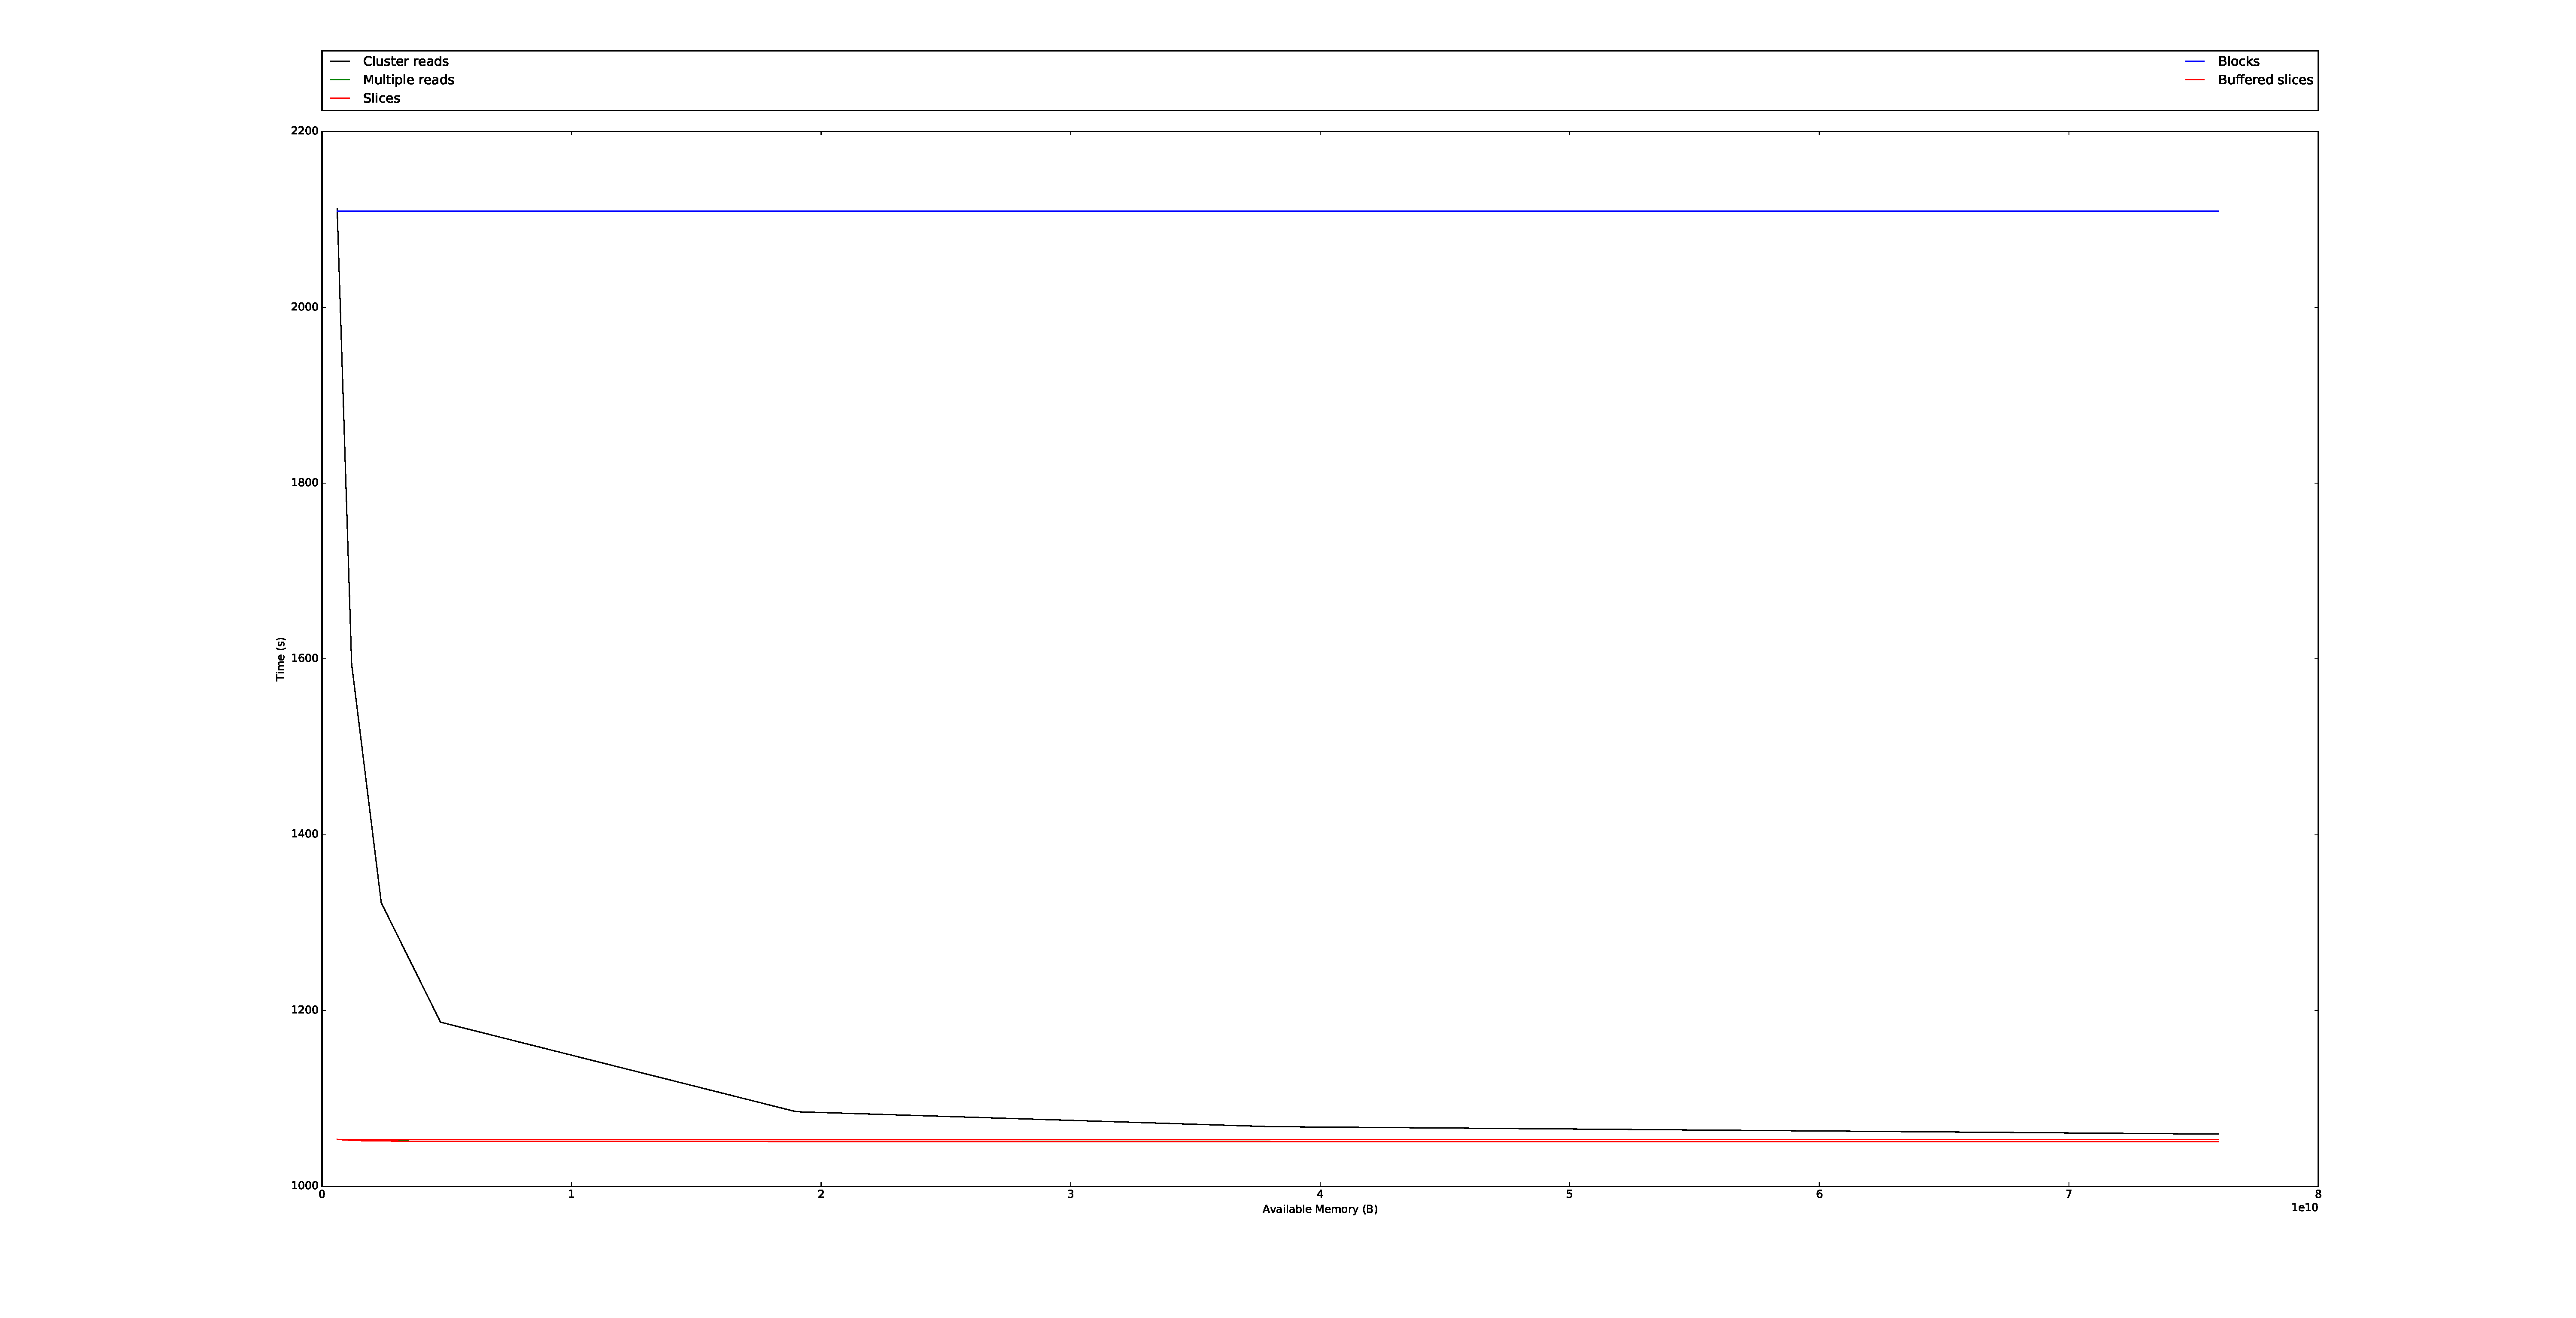
\includegraphics[width=\columnwidth]{figures/model.pdf}
  % see function.py
  \caption{Model comparison}
  \label{fig:models}
\end{figure}
\todo{redraw the figure. Benchmark $\alpha$ and $\beta$ more
  accurately on the HDD or SSD. In the previous sections, compare the
  model with real experiments, to validate the model.}

\subsection{Lossless Compression}

\subsection{Splitting}


\section{Discussion}
\label{sec:discussion}

What is the best algorithm (between 3 and 4), in which context. Did we
solve the seek problem or is there any issue remaining?

File formats:
\begin{itemize}
\item would MINC~\cite{vincent2016minc} support such algorithms? See on-going email discussion
with P. Bellec.
\item some formats optimize the storage for particular split shapes. See
  ndstore~\cite{burns2013open}. Such formats would behave equally
  poorly with chunks that do not comply to this geometry. Our
  algorithms would work equally well with such formats.
\end{itemize}

The performance model might be dependent on the particular
infrastructure (disks, OS and filesystem) used in the experiments. In
particular, caching might behave differently in a different setup.

Reconstructing (therefore splitting) a complete 3D image may not
always be necessary. Re-splitting, for instance, could be done from
existing chunks.

\section{Conclusion}

Future work:
- obliques
- parallel algorithms
- re-splitting
- model

\section*{Acknowledgment}

(If not added as co-authors): Greg Kiar, Pierre Bellec.

\bibliographystyle{IEEEtran}
\bibliography{IEEEabrv,biblio.bib}

\end{document}
